% presentasi_data_analitik.tex
% Presentasi Tugas Data Analitik — C-MAPSS RUL Prediction
% Departemen Teknik Mesin FTUI — 2026
% Theme: light, clean, UI blue accents

\documentclass[aspectratio=169, 11pt]{beamer}

% ── Packages ──────────────────────────────────────────────────────────────────
\usepackage[T1]{fontenc}
\usepackage[utf8]{inputenc}
\usepackage{graphicx}
\usepackage{booktabs}
\usepackage{amsmath}
\usepackage{xcolor}
\usepackage{tikz}
\usepackage{subcaption}

% ── Colors ────────────────────────────────────────────────────────────────────
\definecolor{uiblue}{RGB}{0,56,147}
\definecolor{uibluelight}{RGB}{220,230,248}
\definecolor{uiteal}{RGB}{15,110,86}
\definecolor{uicoral}{RGB}{153,60,29}
\definecolor{uigray}{RGB}{100,100,100}
\definecolor{bglight}{RGB}{250,251,253}

% ── Beamer theme ──────────────────────────────────────────────────────────────
\usetheme{default}
\usecolortheme{default}
\setbeamercolor{normal text}{fg=black, bg=white}
\setbeamercolor{frametitle}{fg=uiblue, bg=uibluelight}
\setbeamercolor{title}{fg=white, bg=uiblue}
\setbeamercolor{subtitle}{fg=white}
\setbeamercolor{author}{fg=white}
\setbeamercolor{institute}{fg=white}
\setbeamercolor{date}{fg=white}
\setbeamercolor{block title}{fg=white, bg=uiblue}
\setbeamercolor{block body}{fg=black, bg=uibluelight}
\setbeamercolor{itemize item}{fg=uiblue}
\setbeamercolor{itemize subitem}{fg=uiteal}
\setbeamercolor{enumerate item}{fg=uiblue}
\setbeamercolor{footline}{fg=uigray}
\setbeamercolor{structure}{fg=uiblue}

\setbeamerfont{frametitle}{size=\large, series=\bfseries}
\setbeamerfont{title}{size=\Large, series=\bfseries}
\setbeamerfont{block title}{size=\normalsize, series=\bfseries}

% remove navigation symbols
\setbeamertemplate{navigation symbols}{}

% footer
\setbeamertemplate{footline}{
  \leavevmode
  \hbox{
    \begin{beamercolorbox}[wd=.6\paperwidth, ht=2.2ex, dp=1ex, left,
        leftskip=4mm]{footline}
      \footnotesize\color{uigray}
      Prediksi RUL Mesin Turbofan C-MAPSS --- Data Analitik 2026
    \end{beamercolorbox}
    \begin{beamercolorbox}[wd=.4\paperwidth, ht=2.2ex, dp=1ex, right,
        rightskip=4mm]{footline}
      \footnotesize\color{uigray}
      \insertframenumber{} / \inserttotalframenumber
    \end{beamercolorbox}
  }
  \vskip0pt
}

% frametitle with left bar
\setbeamertemplate{frametitle}{
  \vspace{0.15cm}
  
\begin{tikzpicture}[remember picture, overlay]
    \fill[uiblue] (0, 0.05) rectangle (0.06, 0.55);
  \end{tikzpicture}
  \hspace{0.15cm}
  \insertframetitle
  \vspace{0.05cm}
}

% itemize bullets
\setbeamertemplate{itemize item}{\color{uiblue}\textbullet}
\setbeamertemplate{itemize subitem}{\color{uiteal}$\circ$}

% ── Title info ─────────────────────────────────────────────────────────────────
\title{Prediksi \textit{Remaining Useful Life}\\
       Mesin Turbofan Menggunakan ANN\\
       pada Dataset C-MAPSS}
\subtitle{Tugas Data Analitik}
\author{
  Luqman Alifio Arhab \and
  Azfa Rhazasta Abiandra \\
  Adamsyah Haryo Saksono \and
  Epsiarto Rizqi Nurwijayadi
}
\institute{Departemen Teknik Mesin FTUI}
\date{2026}

% ══════════════════════════════════════════════════════════════════════════════
\begin{document}

% ── Slide 1: Cover ────────────────────────────────────────────────────────────
\begin{frame}[plain]
  \setbeamercolor{background canvas}{bg=uiblue}
  \centering
  \vspace{0.4cm}
  
\includegraphics[height=1.3cm]{images/logo_ui.png}

  \vspace{0.2cm}
  {\color{white}\small Universitas Indonesia ---
    Departemen Teknik Mesin FTUI\par}

  \vspace{0.3cm}
  {\color{uibluelight}\rule{0.8\textwidth}{0.4pt}\par}
  \vspace{0.2cm}

  {\color{white}\LARGE\bfseries
    Prediksi \textit{Remaining Useful Life}\\[0.2em]
    Mesin Turbofan Menggunakan ANN\\[0.2em]
    pada Dataset C-MAPSS\par}

  \vspace{0.3cm}
  {\color{uibluelight}\rule{0.8\textwidth}{0.4pt}\par}
  \vspace{0.3cm}

  {\color{white!80}\small
    Luqman Alifio Arhab \quad Azfa Rhazasta Abiandra \\[0.2em]
    Adamsyah Haryo Saksono \quad Epsiarto Rizqi Nurwijayadi\par}

  \vspace{0.2cm}
  {\color{white!70}\footnotesize Data Analitik --- 2026\par}
\end{frame}

% ── Slide 2: Outline ─────────────────────────────────────────────────────────
\begin{frame}{Outline}
  \begin{columns}[t]
    \begin{column}{0.48\textwidth}
      \begin{block}{Analisis Data}
        \begin{enumerate}
          \item Dataset C-MAPSS
          \item Pembersihan Data
          \item Normalisasi
          \item Seleksi Fitur (Pearson + PCA)
        \end{enumerate}
      \end{block}
    \end{column}
    \begin{column}{0.48\textwidth}
      \begin{block}{Pemodelan}
        \begin{enumerate}[start=5]
          \item Model ANN (Python + MATLAB)
          \item Benchmark 8 Model
          \item Analisis Garson
          \item Perbandingan Python vs MATLAB
          \item Kesimpulan
        \end{enumerate}
      \end{block}
    \end{column}
  \end{columns}

  \vspace{0.4cm}
  \centering\small
  \begin{beamercolorbox}[sep=4pt]{block body}
\color{uiblue}
      Raw .txt $\rightarrow$ HDF5/CSV $\rightarrow$ Cleaning
      $\rightarrow$ Normalisasi $\rightarrow$ PCA
      $\rightarrow$ \textbf{ANN} $\rightarrow$ Garson
\end{beamercolorbox}
\end{frame}

% ── Slide 3: Latar Belakang ───────────────────────────────────────────────────
\begin{frame}{Latar Belakang}
  \begin{columns}[c]
    \begin{column}{0.50\textwidth}
      \begin{itemize}
        \item \textbf{RUL} (\textit{Remaining Useful Life}) =
          sisa siklus sebelum kegagalan komponen
        \item Digunakan dalam sistem \textbf{PHM}
          (\textit{Prognostics and Health Management})
        \item Tujuan: optimalkan jadwal perawatan,
          kurangi \textit{downtime} tak terencana
        \item Dataset: \textbf{C-MAPSS NASA} ---
          simulasi turbofan dari kondisi sehat hingga gagal
      \end{itemize}

      \vspace{0.3cm}
      \begin{beamercolorbox}[sep=4pt]{block body}
\color{uiblue}\small
          \textbf{Pertanyaan:} Dari pembacaan sensor saat ini,
          berapa siklus tersisa sebelum mesin gagal?
\end{beamercolorbox}
    \end{column}
    \begin{column}{0.46\textwidth}
      
\includegraphics[width=\textwidth]{images/01_phm_ecosystem_stack.png}
    \end{column}
  \end{columns}
\end{frame}

% ── Slide 4: Dataset ─────────────────────────────────────────────────────────
\begin{frame}{Dataset C-MAPSS}
  \begin{columns}[c]
    \begin{column}{0.52\textwidth}
      
\includegraphics[width=\textwidth]{images/09_dataset_matrix.png}
    \end{column}
    \begin{column}{0.44\textwidth}
      \begin{itemize}
        \item \textbf{4 sub-dataset}: FD001--FD004
        \item \textbf{Kondisi operasi}: 1 atau 6
        \item \textbf{Mode kerusakan}: HPC, atau HPC+Fan
        \item \textbf{26 kolom}: unit, cycle,
          3 op\_settings, 21 sensor
        \item \textbf{Train}: siklus penuh hingga gagal
          $\rightarrow$ RUL dapat dihitung
        \item \textbf{Test}: dipotong sebelum gagal
          $\rightarrow$ RUL harus diprediksi
      \end{itemize}
      \vspace{0.2cm}
      \centering
      
\includegraphics[width=0.85\textwidth]{images/10_train_test_rul_relationship.png}
    \end{column}
  \end{columns}
\end{frame}

% ── Slide 5: Engine + Degradasi ───────────────────────────────────────────────
\begin{frame}{Struktur Mesin dan Sinyal Degradasi}
  \begin{columns}[c]
    \begin{column}{0.54\textwidth}
      
\includegraphics[width=\textwidth]{images/03_cmapss_engine_schematic.png}
      \vspace{0.1cm}
      \centering\footnotesize
      \color{uigray}21 sensor mengukur kondisi sepanjang aliran udara
    \end{column}
    \begin{column}{0.44\textwidth}
      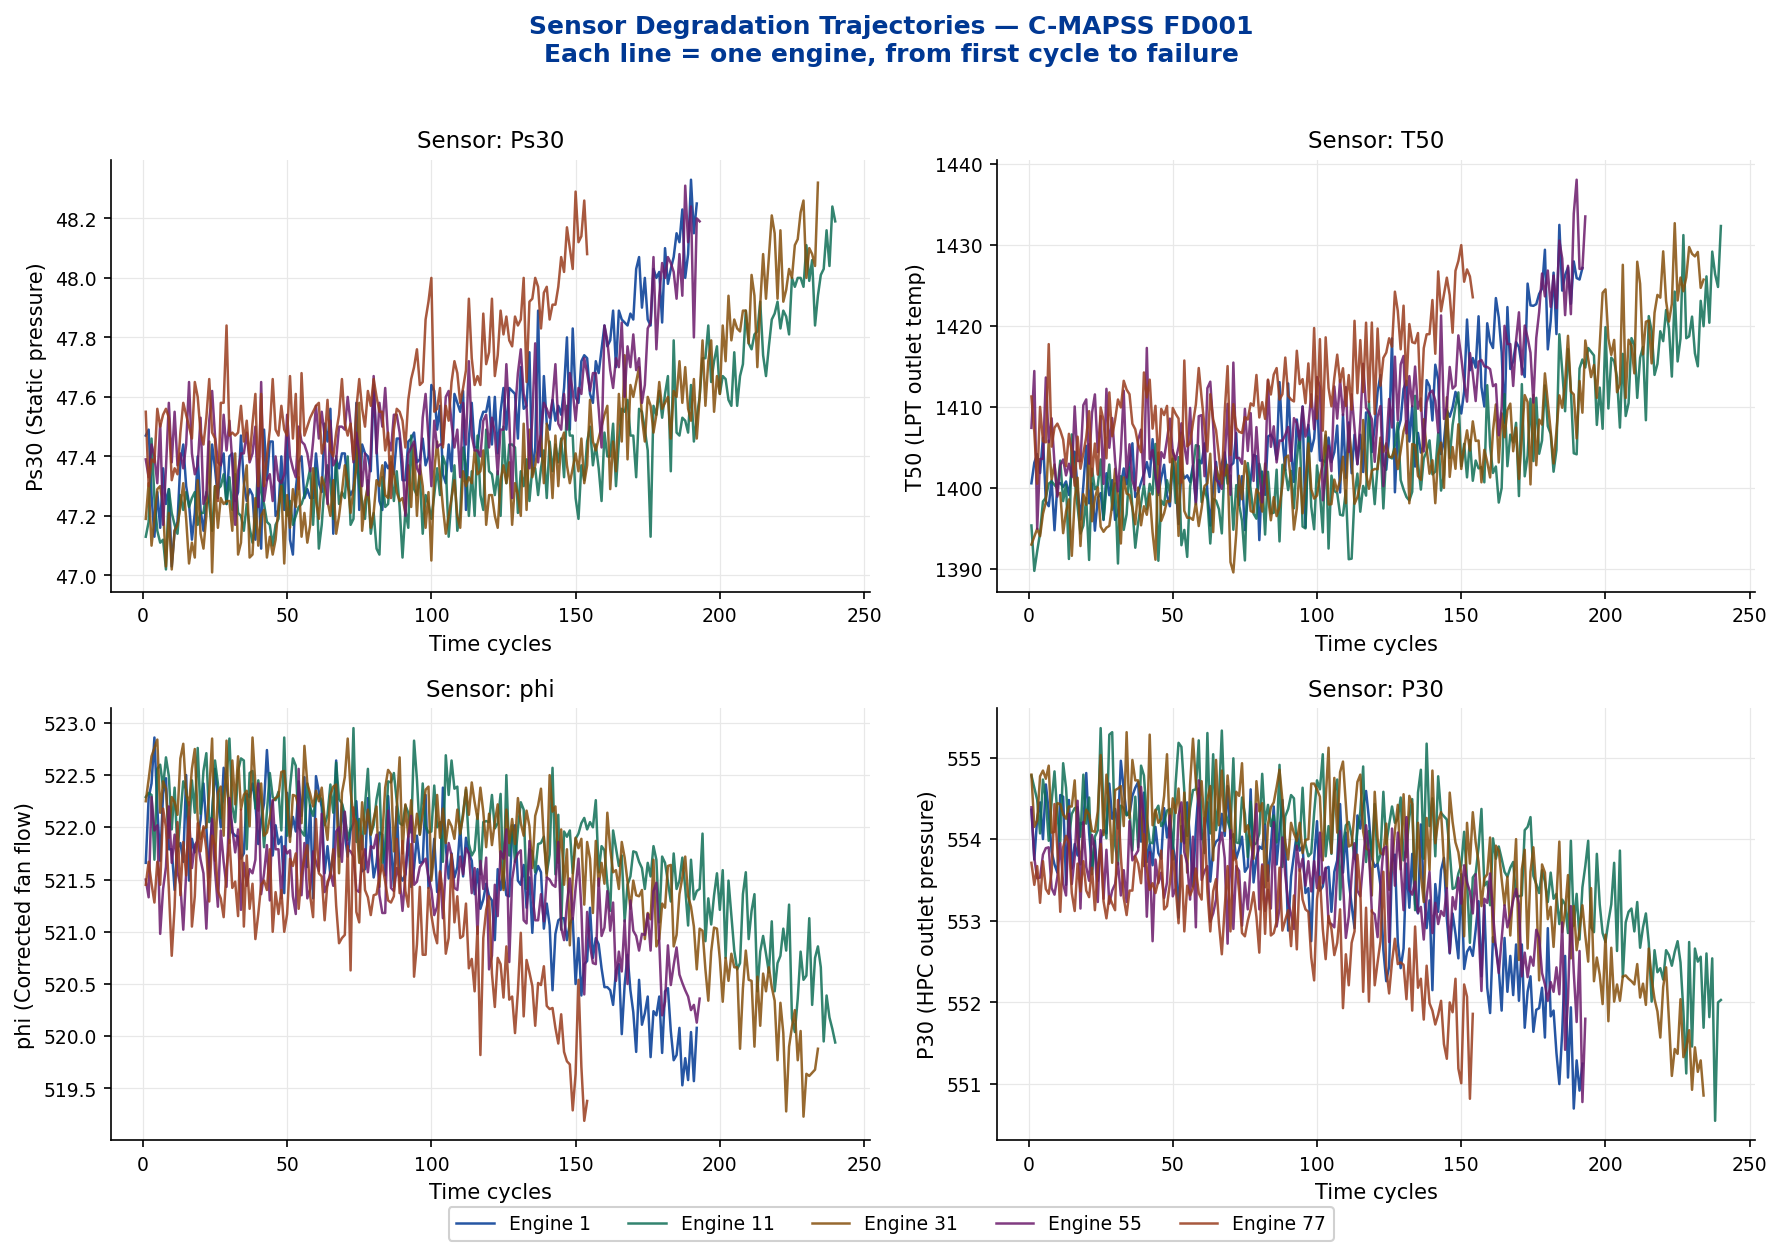
\includegraphics[width=\textwidth]{images/plot_A1_degradation.png}
      \centering\footnotesize
      \color{uigray}Sensor \textit{drift} menjelang kegagalan
    \end{column}
  \end{columns}
\end{frame}

% ── Slide 6: Data Cleaning ────────────────────────────────────────────────────
\begin{frame}{Pembersihan Data}
  \begin{columns}[t]
    \begin{column}{0.48\textwidth}
      \textbf{5 Metode Analisis:}
      \begin{enumerate}
        \item Standar deviasi (std)
        \item Koefisien variasi (CV)
        \item Korelasi Pearson vs RUL
        \item Korelasi Spearman vs RUL
        \item Mutual Information vs RUL
      \end{enumerate}

      \vspace{0.3cm}
      \textbf{Hasil per sub-dataset:}
      \vspace{0.1cm}

      \small
      \begin{tabular}{lcc}
        \toprule
        Sub-dataset & Dihapus & Sensor Aktif \\
        \midrule
        FD001 & 6 & 15 \\
        FD002 & 0 & 21 \\
        FD003 & 5 & 16 \\
        FD004 & 0 & 21 \\
        \bottomrule
      \end{tabular}
    \end{column}
    \begin{column}{0.48\textwidth}
      \begin{beamercolorbox}[sep=4pt]{block body}
\color{uiblue}\small
          \textbf{Sensor dieliminasi FD001:}\\
          T2, P2, epr, farB, Nf\_dmd, PCNfR\_dmd\\[4pt]
          Alasan: std $= 0$ $\Rightarrow$
          Pearson/Spearman = NaN\\[4pt]
          \textbf{FD002/FD004}: tidak ada eliminasi
          karena 6 kondisi membuat semua sensor bervariasi
\end{beamercolorbox}

      \vspace{0.3cm}
      \begin{beamercolorbox}[sep=4pt]{block body}
\color{uiteal}\small
          \textbf{Catatan P15}:
          Pearson = $-0{,}13$ (hampir nol)
          $\Rightarrow$ dieliminasi dari FD001.
          Namun Garson menemukan sinyal non-linear
          yang tersembunyi.
\end{beamercolorbox}
    \end{column}
  \end{columns}
\end{frame}

% ── Slide 7: Normalisasi ──────────────────────────────────────────────────────
\begin{frame}{Normalisasi --- Z-Score Berbasis Siklus Sehat}
  \begin{columns}[c]
    \begin{column}{0.38\textwidth}
      \textbf{Formula:}
      \[
        z = \frac{x - \mu_{c,\,\text{healthy}}}
                 {\sigma_{c,\,\text{healthy}}}
      \]

      \vspace{0.2cm}
      \textbf{Tiga prinsip:}
      \begin{enumerate}
        \item Parameter dari siklus \textit{healthy}
          (RUL $\geq$ 125) saja
        \item Per kondisi operasi (bukan global)
        \item Parameter \textit{train} diterapkan
          ke \textit{test} --- hindari \textit{data leakage}
      \end{enumerate}

      \vspace{0.2cm}
      \small\color{uigray}
      Hasil: $z \approx 0$ = sehat,
      $z$ menyimpang = terdegradasi
    \end{column}
    \begin{column}{0.59\textwidth}
      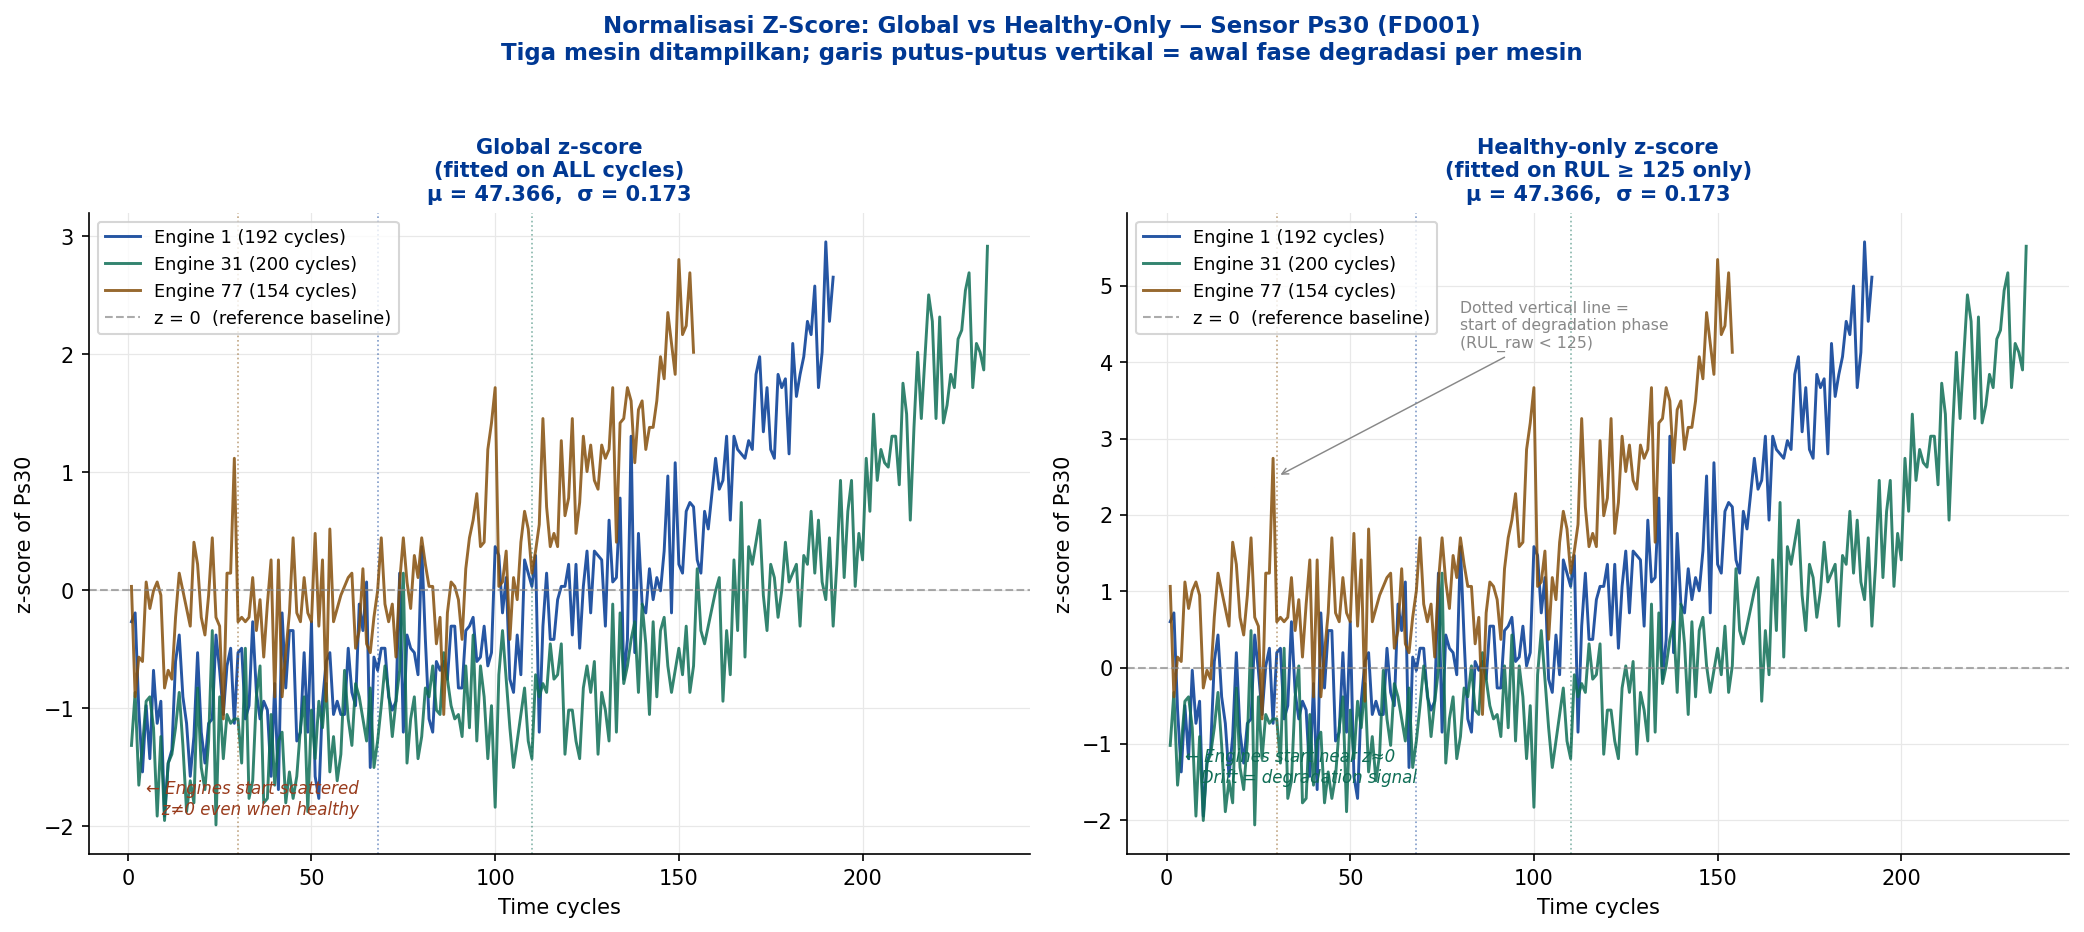
\includegraphics[width=\textwidth]{images/plot_D13_norm_comparison.png}
      \centering\footnotesize\color{uigray}
      Kanan: ketiga mesin mulai di $z \approx 0$,
      \textit{drift} seiring degradasi
    \end{column}
  \end{columns}
\end{frame}

% ── Slide 8: Pearson + PCA Scree ──────────────────────────────────────────────
\begin{frame}{Seleksi Fitur --- Pearson \& PCA}
  \begin{columns}[c]
    \begin{column}{0.48\textwidth}
      \centering
      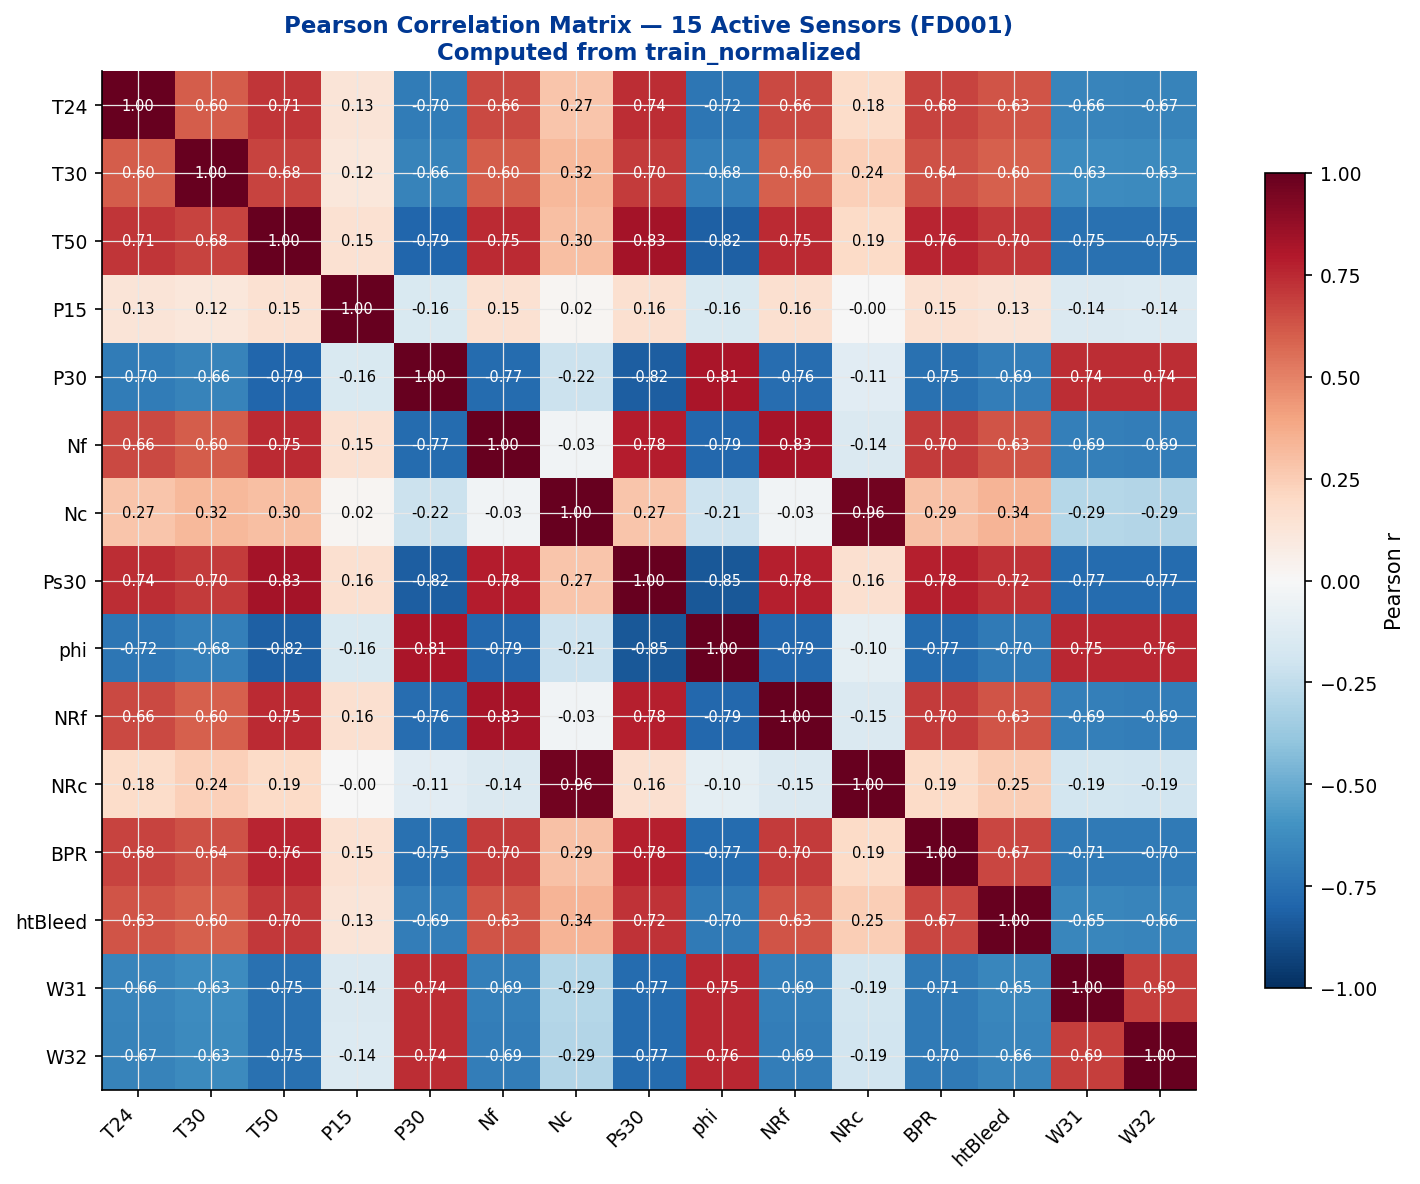
\includegraphics[width=\textwidth]{images/plot_A2_correlation.png}
      \footnotesize\color{uigray}
      Korelasi Pearson --- Nc--NRc $r = 0{,}96$
      (redundansi tinggi $\Rightarrow$ motivasi PCA)
    \end{column}
    \begin{column}{0.48\textwidth}
      \centering
      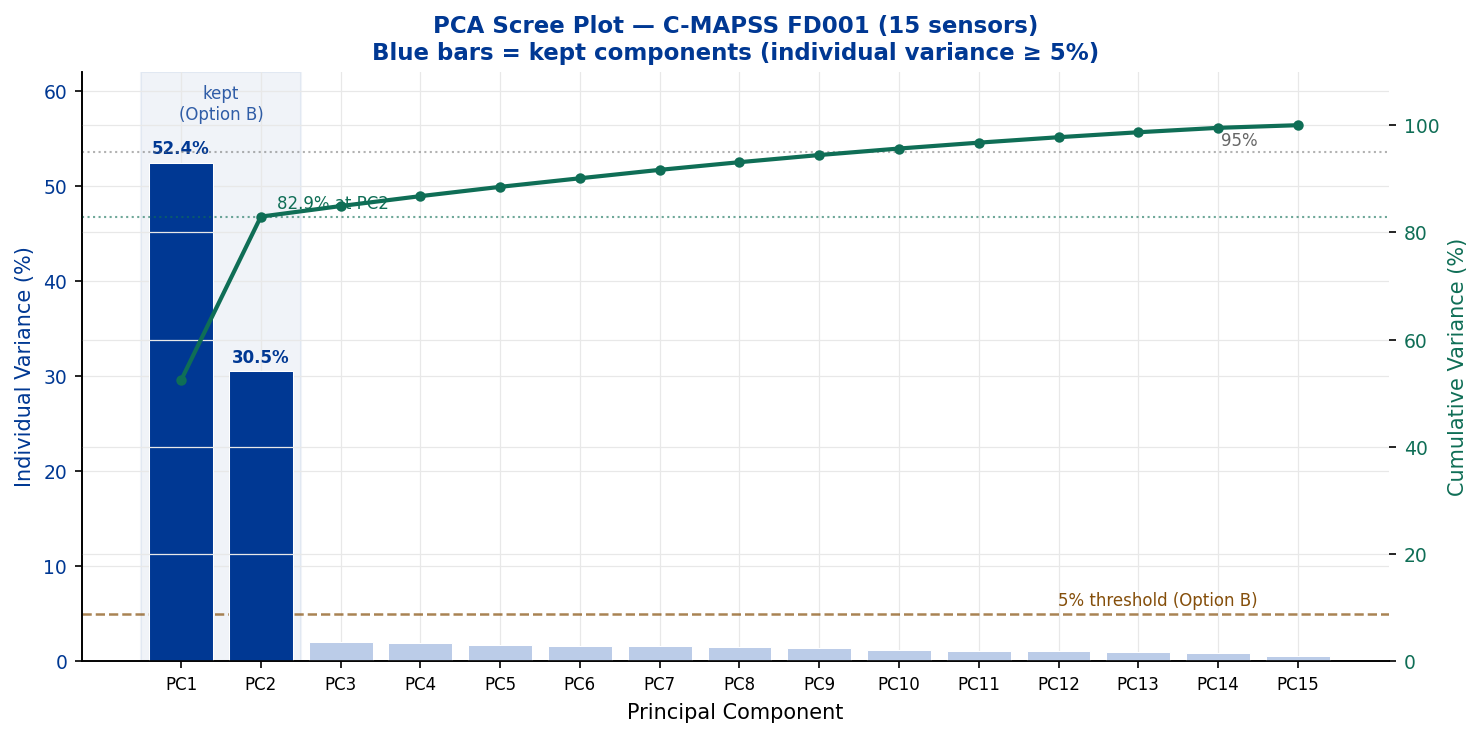
\includegraphics[width=\textwidth]{images/plot_A3_scree.png}
      \footnotesize\color{uigray}
      Scree plot --- \textit{cliff} setelah PC2;
      2 komponen = 82,9\% varians
    \end{column}
  \end{columns}
\end{frame}

% ── Slide 9: PCA Scatter ──────────────────────────────────────────────────────
\begin{frame}{PCA --- Separasi Sehat vs Terdegradasi}
  \begin{columns}[c]
    \begin{column}{0.54\textwidth}
      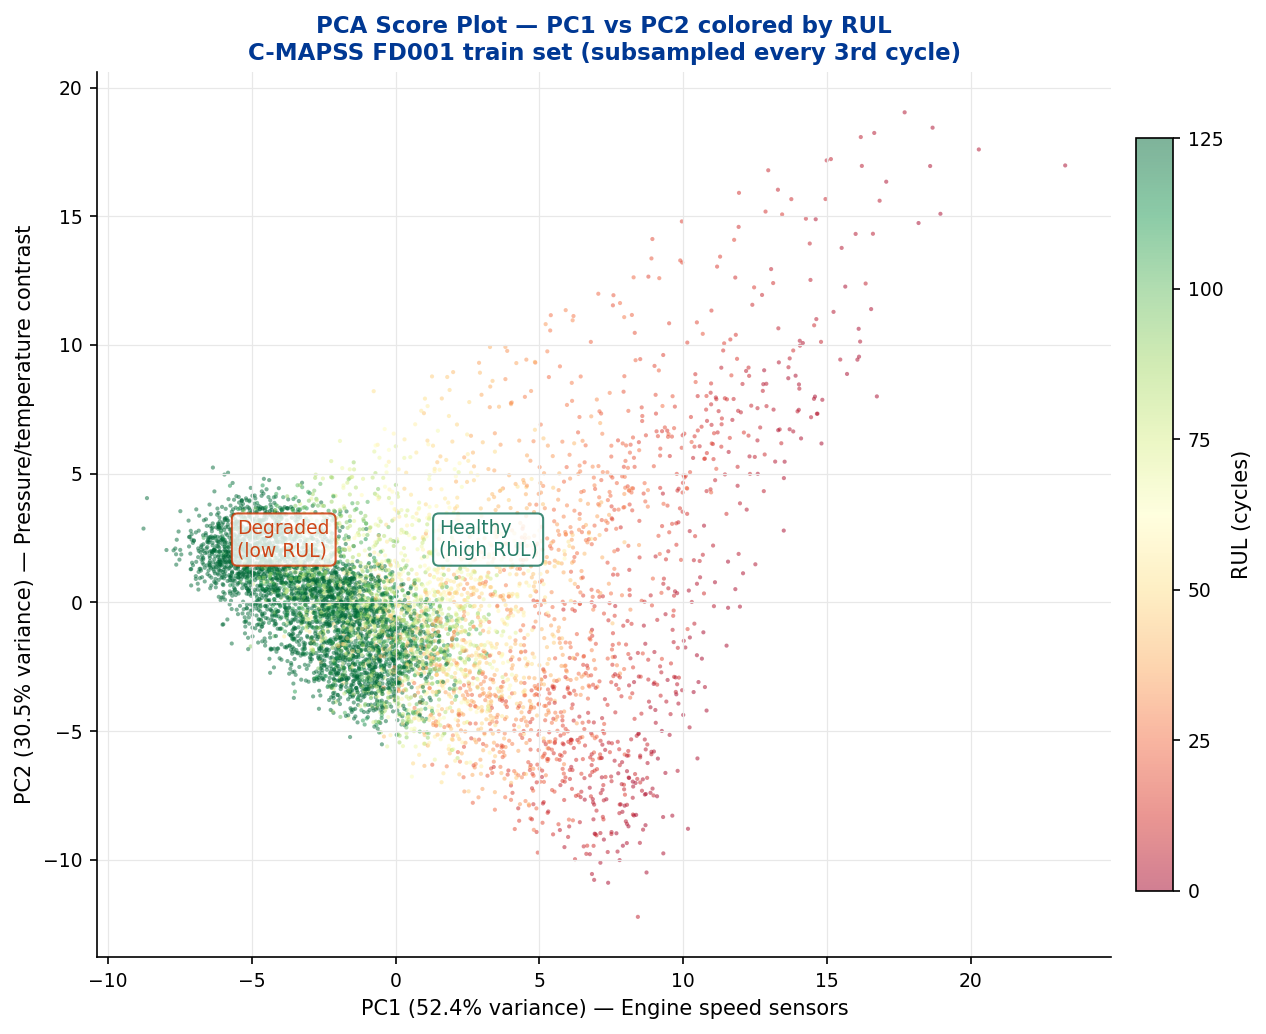
\includegraphics[width=\textwidth]{images/plot_A4_pca_scatter.png}
    \end{column}
    \begin{column}{0.43\textwidth}
      \begin{itemize}
        \item Setiap titik = satu siklus mesin
        \item \textbf{Warna} = RUL (pseudo-Z-axis)
        \item Hijau (sehat) $\rightarrow$ kanan
        \item Merah (degraded) $\rightarrow$ kiri
      \end{itemize}

      \vspace{0.3cm}
      \small
      \begin{tabular}{lcc}
        \toprule
        Dataset & Komp. & Kumulatif \\
        \midrule
        FD001 & 2 & 82,9\% \\
        FD002 & 4 & 74,8\% \\
        FD003 & 3 & 87,8\% \\
        FD004 & 3 & 77,5\% \\
        \bottomrule
      \end{tabular}

      \vspace{0.3cm}
      \begin{beamercolorbox}[sep=4pt]{block body}
\color{uiblue}\small
          PC1 = kecepatan poros (Nf, NRf, Nc, NRc)\\
          PC2 = kontras tekanan-kecepatan
\end{beamercolorbox}
    \end{column}
  \end{columns}
\end{frame}

% ── Slide 10: ANN Arsitektur ──────────────────────────────────────────────────
\begin{frame}{Model ANN --- Arsitektur MLP}
  \begin{columns}[c]
    \begin{column}{0.40\textwidth}
      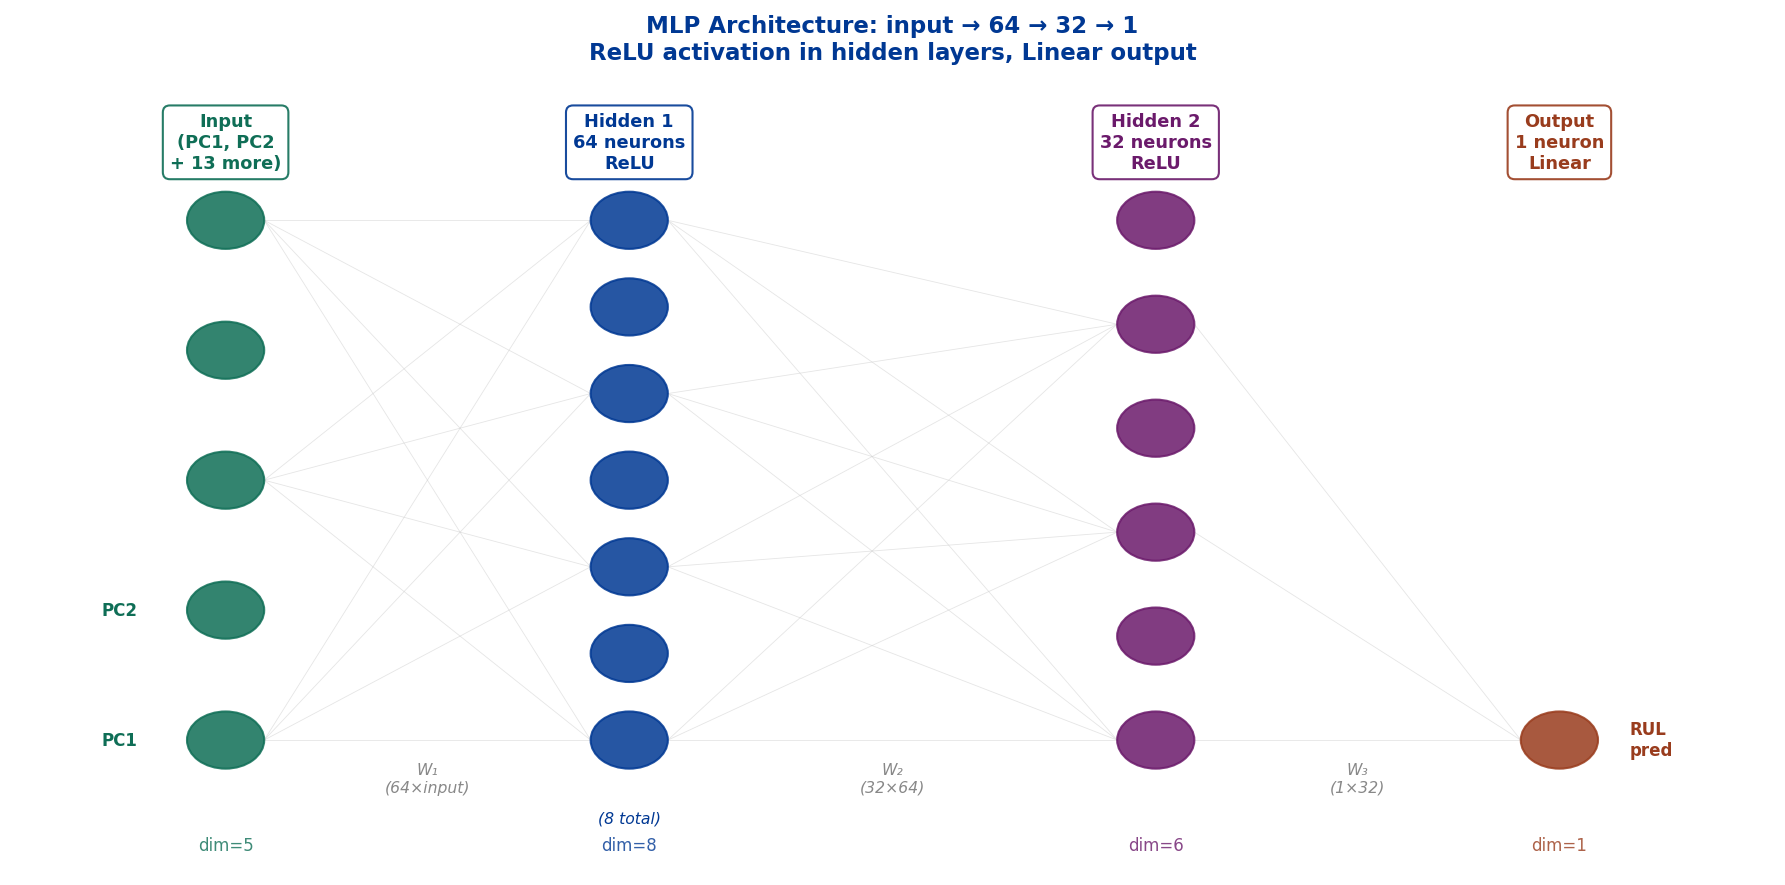
\includegraphics[width=\textwidth]{images/plot_D14_mlp_arch.png}
    \end{column}
    \begin{column}{0.56\textwidth}
      \begin{block}{Konfigurasi}
        \small
        \begin{tabular}{ll}
          Arsitektur & input $\to$ 64 $\to$ 32 $\to$ 1 \\
          Target     & RUL\_capped (cap = 125) \\
          Epoch      & 500 \\
          Batch      & 512 \\
          \hline
          Python     & Adam, ReLU \\
          MATLAB     & trainscg, tansig \\
        \end{tabular}
      \end{block}

      \vspace{0.2cm}
      \begin{columns}[c]
        \begin{column}{0.48\textwidth}
          \centering
          
\includegraphics[width=\textwidth]{images/matlab_arch_pca.png}
          \footnotesize PCA (input=2)
        \end{column}
        \begin{column}{0.48\textwidth}
          \centering
          
\includegraphics[width=\textwidth]{images/matlab_arch_norm.png}
          \footnotesize NORM (input=15)
        \end{column}
      \end{columns}
    \end{column}
  \end{columns}
\end{frame}

% ── Slide 11: RUL Cap + NASA Score ────────────────────────────────────────────
\begin{frame}{RUL Cap dan NASA Score}
  \begin{columns}[c]
    \begin{column}{0.50\textwidth}
      \centering
      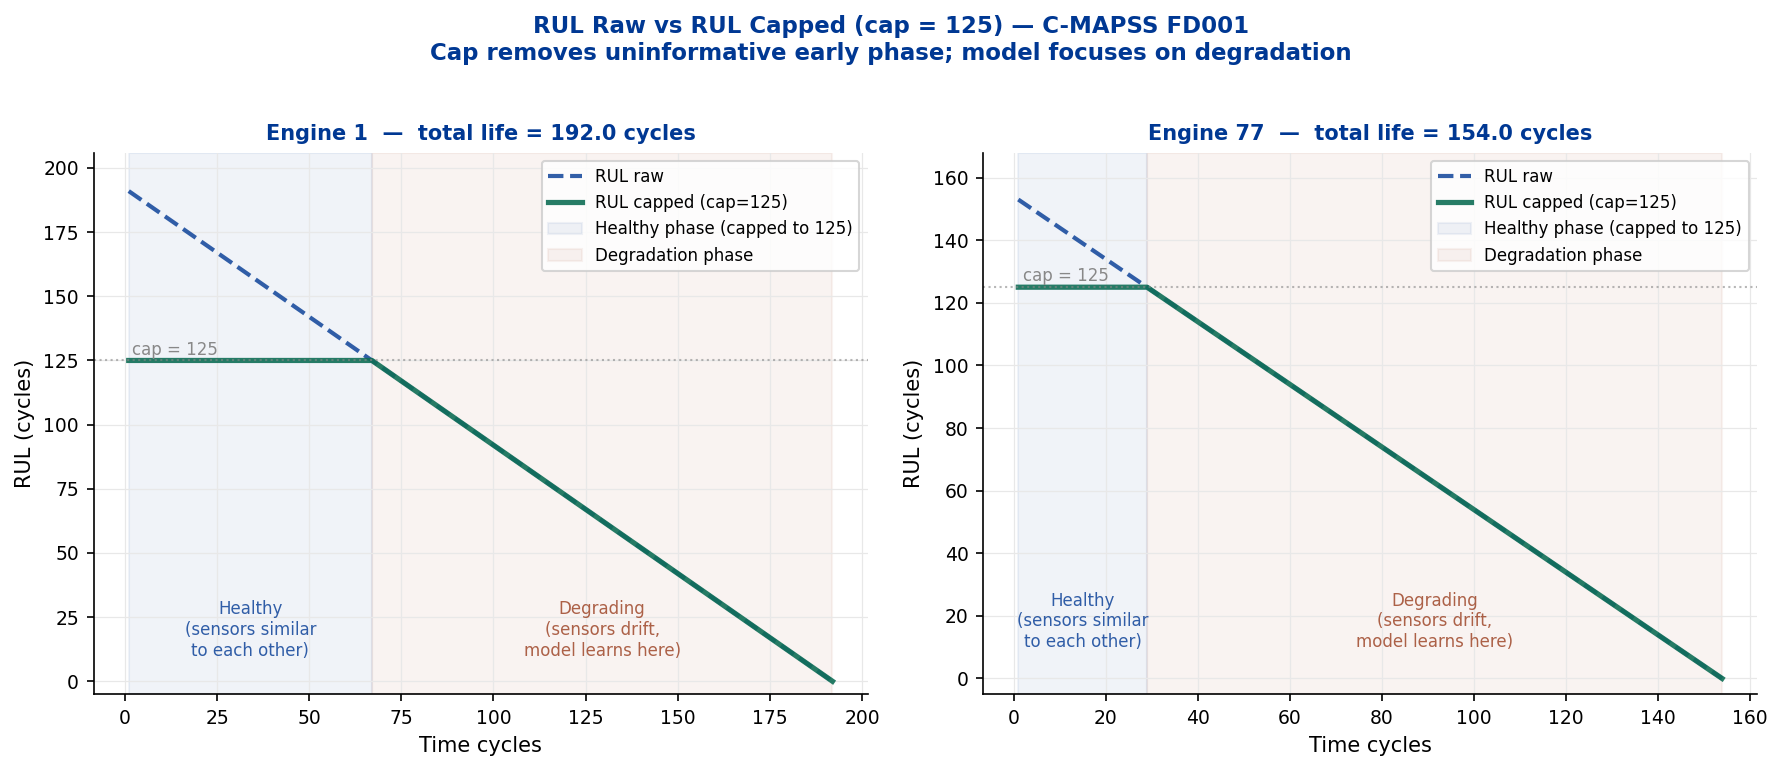
\includegraphics[width=\textwidth]{images/plot_D12_rul_cap.png}
      \footnotesize\color{uigray}
      Cap = 125: fase sehat diratakan;
      model fokus pada fase degradasi
    \end{column}
    \begin{column}{0.47\textwidth}
      \centering
      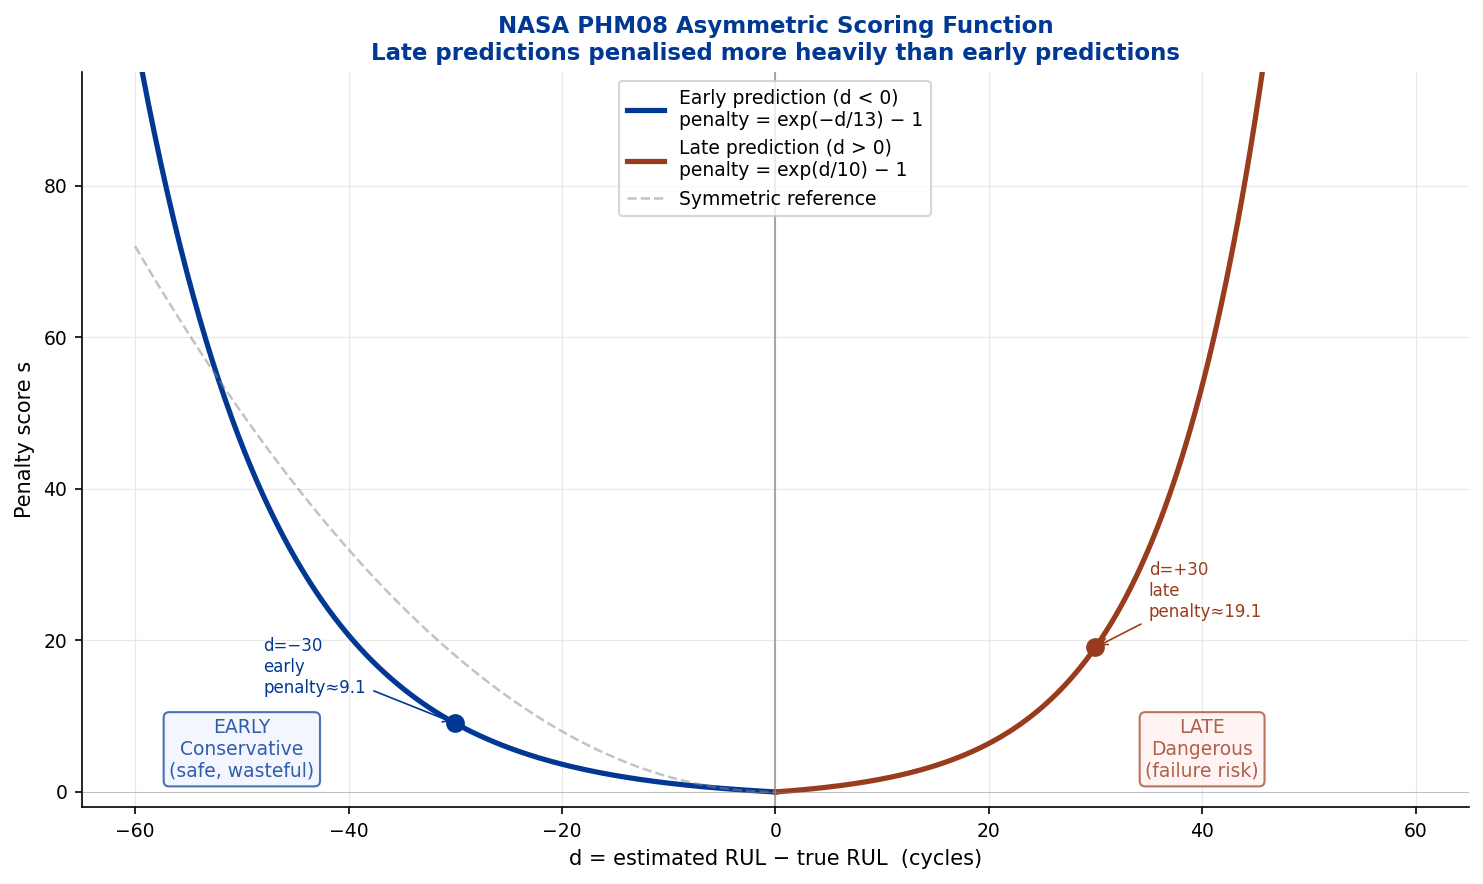
\includegraphics[width=\textwidth]{images/plot_D11_nasa_score.png}
      \footnotesize\color{uigray}
      Prediksi \textit{late} dihukum lebih berat
      karena membahayakan keselamatan
    \end{column}
  \end{columns}
\end{frame}

% ── Slide 12: Benchmark Results ───────────────────────────────────────────────
\begin{frame}{Hasil Benchmark --- 8 Model Python}
  \begin{columns}[t]
    \begin{column}{0.50\textwidth}
      \small
      \begin{tabular}{llcrrr}
        \toprule
        Dataset & Input & Dim & RMSE & MAE & NASA \\
        \midrule
        FD001 & \textbf{PCA}  & 2  & \textbf{17,80} & 12,55 & 815 \\
        FD001 & NORM & 15 & 18,21 & 13,52 & 929 \\
        \midrule
        FD002 & \textbf{PCA}  & 4  & \textbf{29,30} & 20,52 & 14.423 \\
        FD002 & NORM & 21 & 29,45 & 20,73 & \textbf{12.990} \\
        \midrule
        FD003 & PCA  & 3  & 21,87 & 16,17 & 2.650 \\
        FD003 & \textbf{NORM} & 16 & \textbf{20,16} & 15,28 & \textbf{1.783} \\
        \midrule
        FD004 & PCA  & 3  & 30,59 & 23,28 & 9.267 \\
        FD004 & \textbf{NORM} & 21 & \textbf{29,68} & 22,38 & \textbf{7.157} \\
        \bottomrule
      \end{tabular}
    \end{column}
    \begin{column}{0.47\textwidth}
      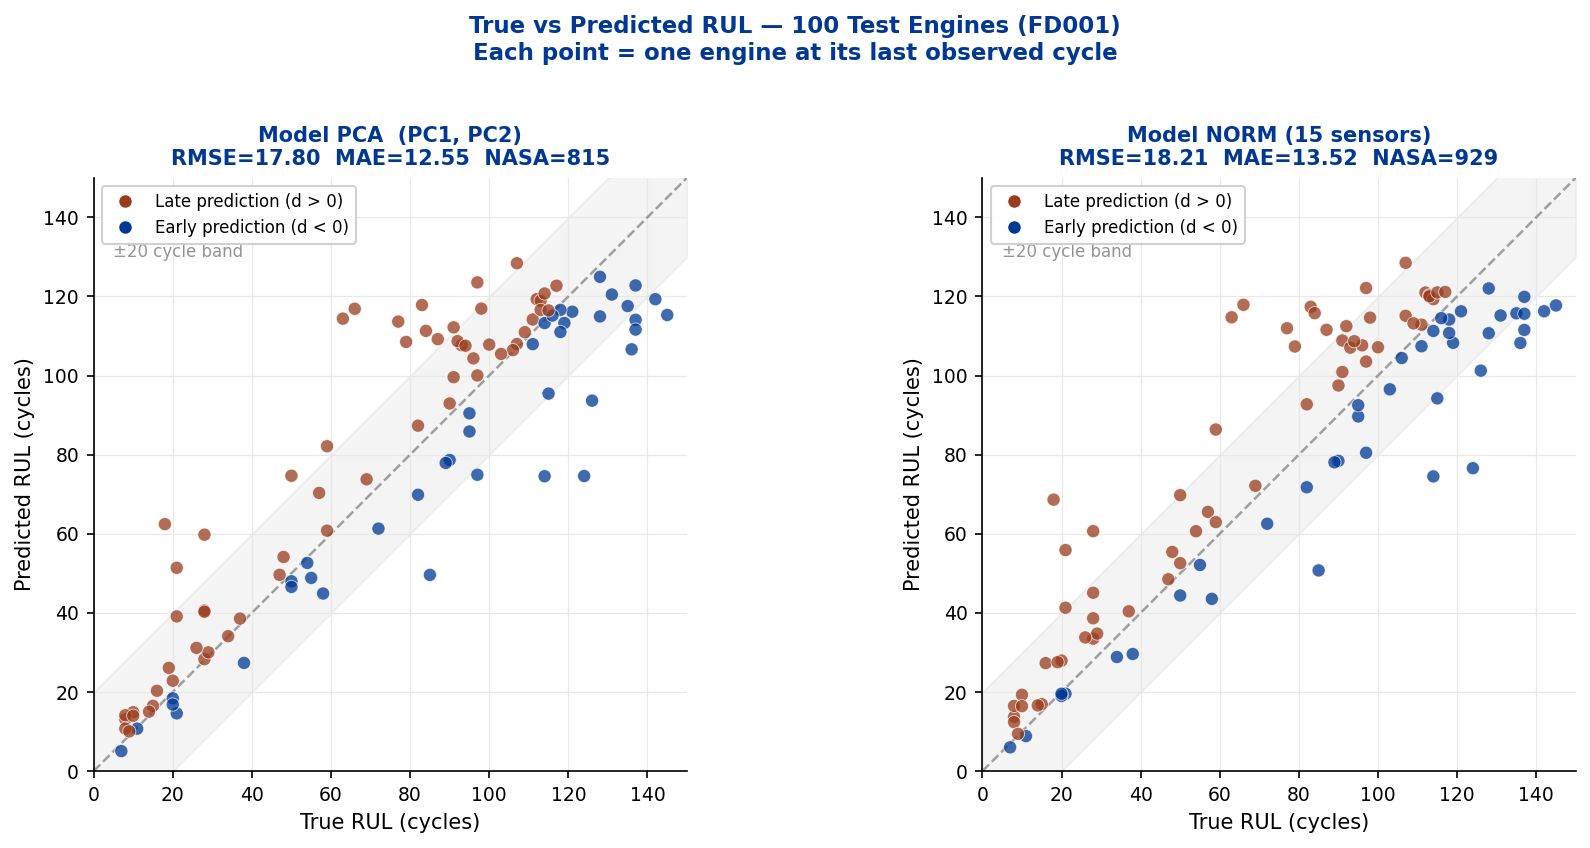
\includegraphics[width=\textwidth]{images/plot_B6_true_vs_pred.png}
      \vspace{0.1cm}

      \begin{beamercolorbox}[sep=4pt]{block body}
\color{uiblue}\footnotesize
          \textbf{Faktor dominan}: kondisi operasi ---
          6 kondisi $\Rightarrow$ RMSE 60\% lebih tinggi\\[3pt]
          \textbf{PCA} lebih baik: dataset sederhana\\
          \textbf{NORM} lebih baik: dataset kompleks
\end{beamercolorbox}
    \end{column}
  \end{columns}
\end{frame}

% ── Slide 13: Garson ─────────────────────────────────────────────────────────
\begin{frame}{Analisis Garson --- Kepentingan Fitur}
  \begin{columns}[c]
    \begin{column}{0.50\textwidth}
      \centering
      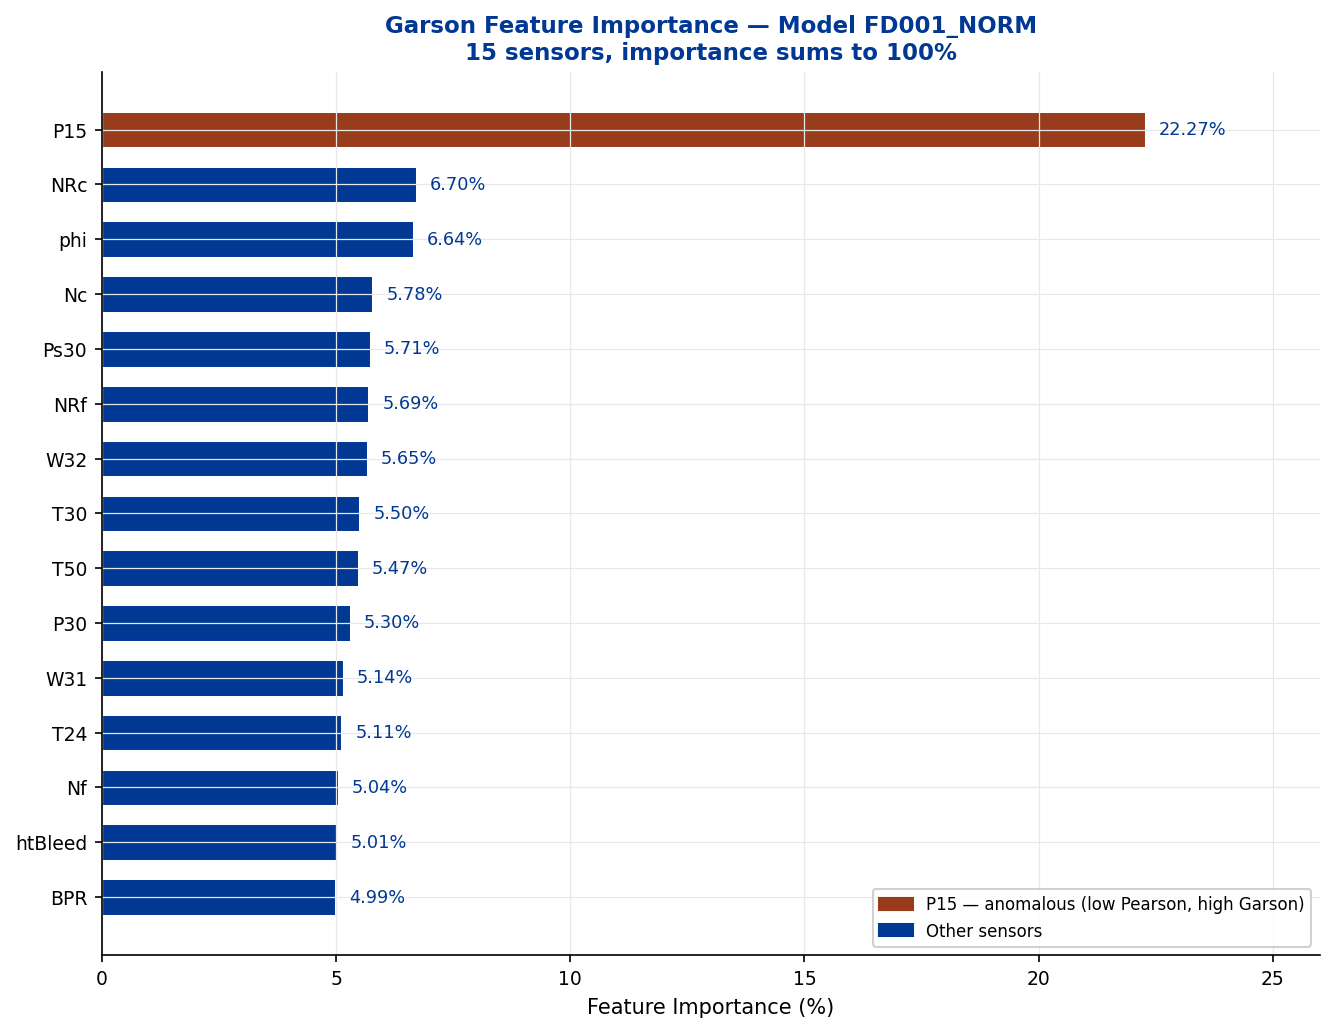
\includegraphics[width=0.90\textwidth]{images/plot_C8_garson_norm.png}
      \footnotesize\color{uigray}
      P15 dominan (22,27\%) meski Pearson = $-0{,}13$
    \end{column}
    \begin{column}{0.47\textwidth}
      \centering
      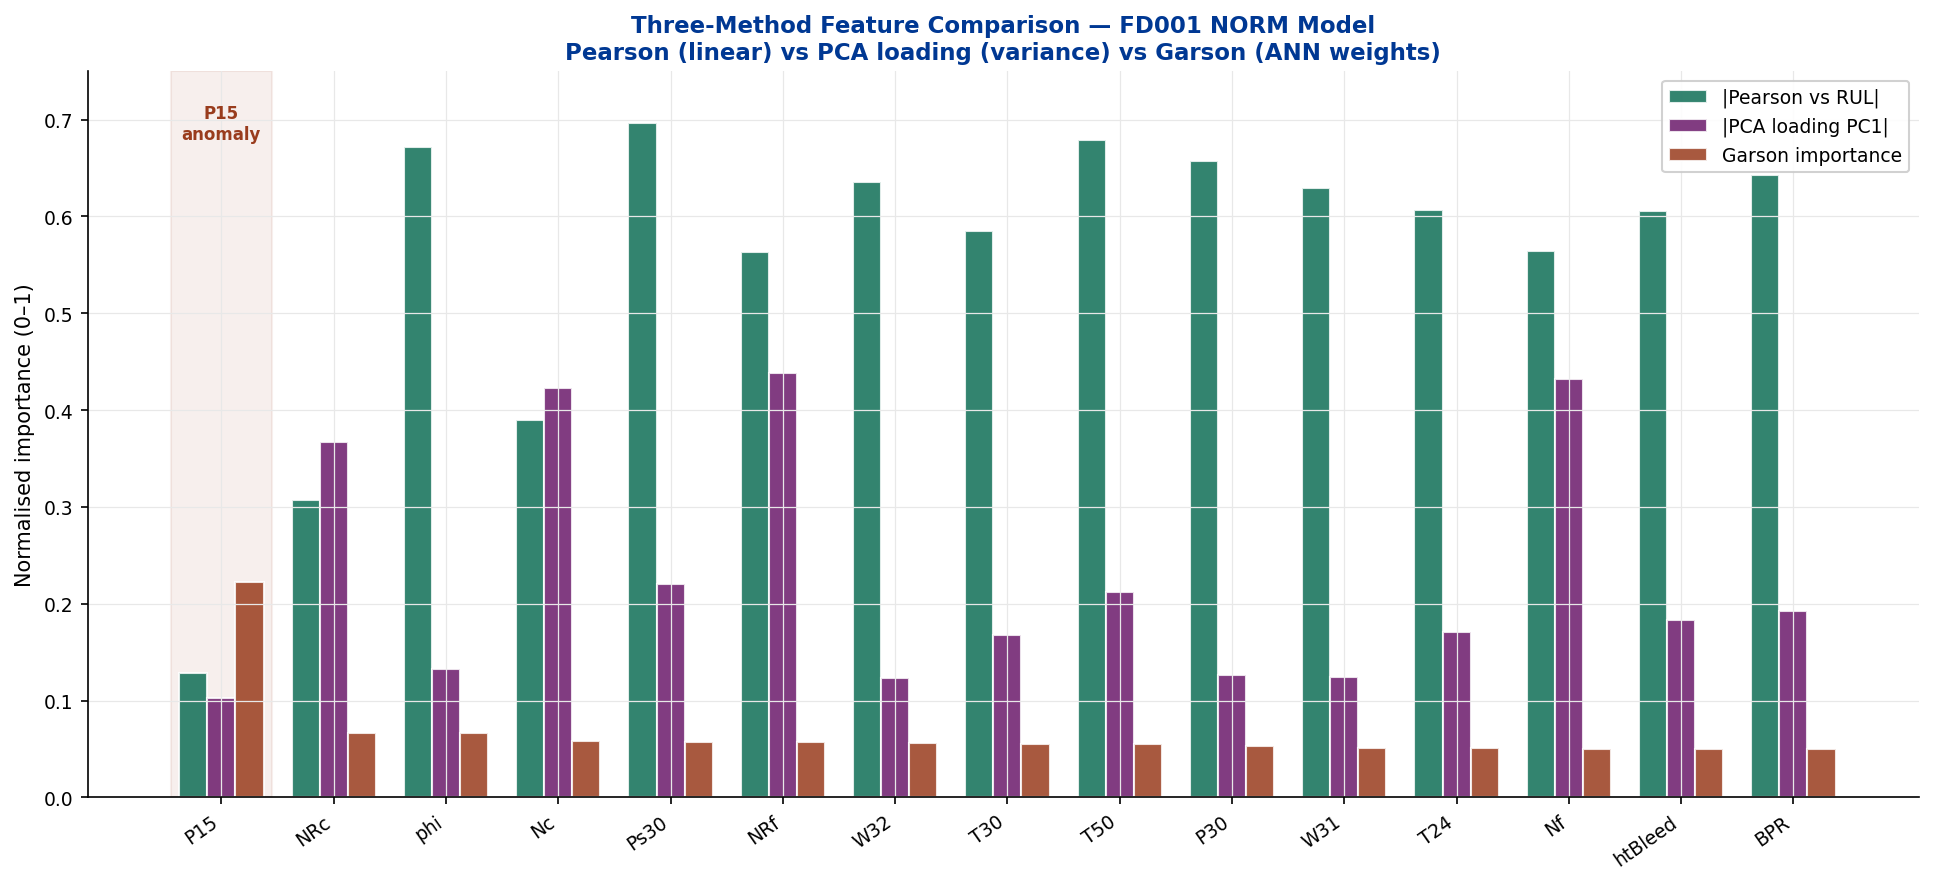
\includegraphics[width=\textwidth]{images/plot_C9_three_method.png}
      \footnotesize\color{uigray}
      Tiga metode: Pearson rendah, PCA rendah,
      Garson tinggi --- ANN menemukan sinyal non-linear
    \end{column}
  \end{columns}
\end{frame}

% ── Slide 14: Python vs MATLAB ────────────────────────────────────────────────
\begin{frame}{Perbandingan Python vs MATLAB}
  \begin{columns}[t]
    \begin{column}{0.48\textwidth}
      \small
      \begin{tabular}{llrrr}
        \toprule
        Impl. & Model & RMSE & MAE & NASA \\
        \midrule
        \textcolor{uiblue}{Python}
          & PCA  & \textbf{17,80} & 12,55 & 815 \\
        \textcolor{uiblue}{Python}
          & NORM & 18,21 & 13,52 & 929 \\
        \midrule
        \textcolor{uiteal}{MATLAB}
          & PCA  & 18,30 & 13,34 & 845 \\
        \textcolor{uiteal}{MATLAB}
          & NORM & 20,91 & 15,75 & 1.319 \\
        \bottomrule
      \end{tabular}

      \vspace{0.2cm}
      \footnotesize
      \textbf{PCA}: selisih $< 3\%$ --- konsisten\\
      \textbf{NORM}: selisih 14,8\% --- ReLU vs tansig

      \vspace{0.2cm}
      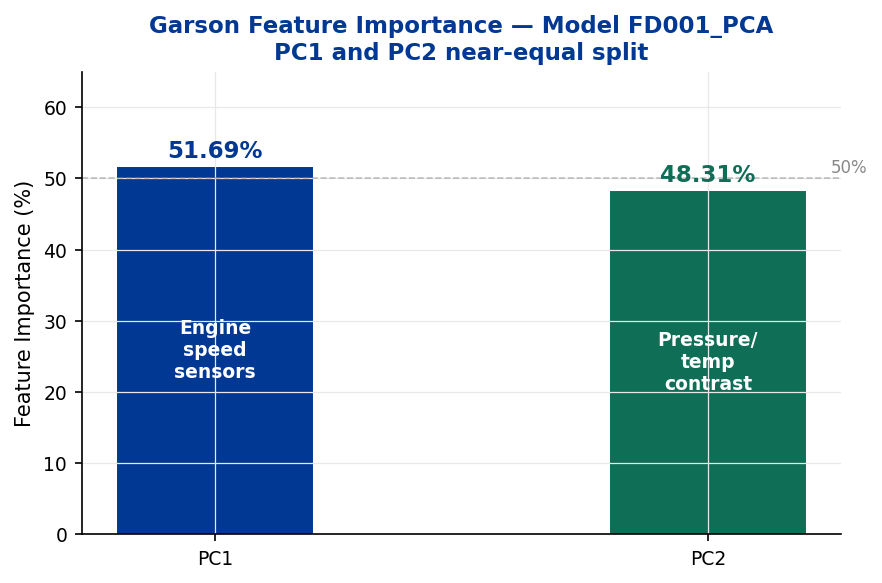
\includegraphics[width=0.48\textwidth]{images/plot_C10_garson_pca.png}
      
\includegraphics[width=0.48\textwidth]{images/matlab_C10_garson_pca.png}\\
      \footnotesize\centering Python \hspace{1.5cm} MATLAB
    \end{column}
    \begin{column}{0.48\textwidth}
      \begin{itemize}
        \item \textbf{Optimizer}: Adam (Python) vs
          trainscg (MATLAB)
        \item \textbf{Aktivasi}: ReLU vs tansig
        \item \textbf{GPU}: PyTorch RTX;
          feedforwardnet CPU only
        \item \textbf{Garson PCA}: konsisten ---
          PC1 $\approx$51\%, PC2 $\approx$49\%
      \end{itemize}

      \vspace{0.2cm}
      \begin{beamercolorbox}[sep=4pt]{block body}
        \footnotesize
        \textbf{Implikasi}: untuk penggunaan nyata,
        Python lebih disarankan karena akurasi lebih
        tinggi dan GPU support.
        MATLAB berguna untuk cross-validation dan
        dokumentasi akademik.
      \end{beamercolorbox}
    \end{column}
  \end{columns}
\end{frame}

% ── Slide 15: Kesimpulan ─────────────────────────────────────────────────────
\begin{frame}{Kesimpulan}
  \begin{columns}[t]
    \begin{column}{0.55\textwidth}
      \begin{enumerate}
        \item \textbf{Kondisi operasi adalah faktor dominan} ---
          6 kondisi $\Rightarrow$ RMSE 60\% lebih tinggi
          dari 1 kondisi

        \vspace{0.15cm}
        \item \textbf{Tipe input optimal} bergantung pada
          kompleksitas: PCA untuk dataset sederhana,
          NORM untuk kompleks

        \vspace{0.15cm}
        \item \textbf{Python (Adam/ReLU) lebih akurat}
          dari MATLAB (trainscg/tansig) terutama
          untuk model NORM

        \vspace{0.15cm}
        \item \textbf{Garson mengungkap sinyal non-linear}
          --- P15 dengan Pearson rendah namun
          penting menurut ANN (22,27\%)

        \vspace{0.15cm}
        \item \textbf{Eliminasi sensor harus per sub-dataset}
          --- sensor konstan di FD001 aktif di FD002
      \end{enumerate}
    \end{column}
    \begin{column}{0.42\textwidth}
      \centering
      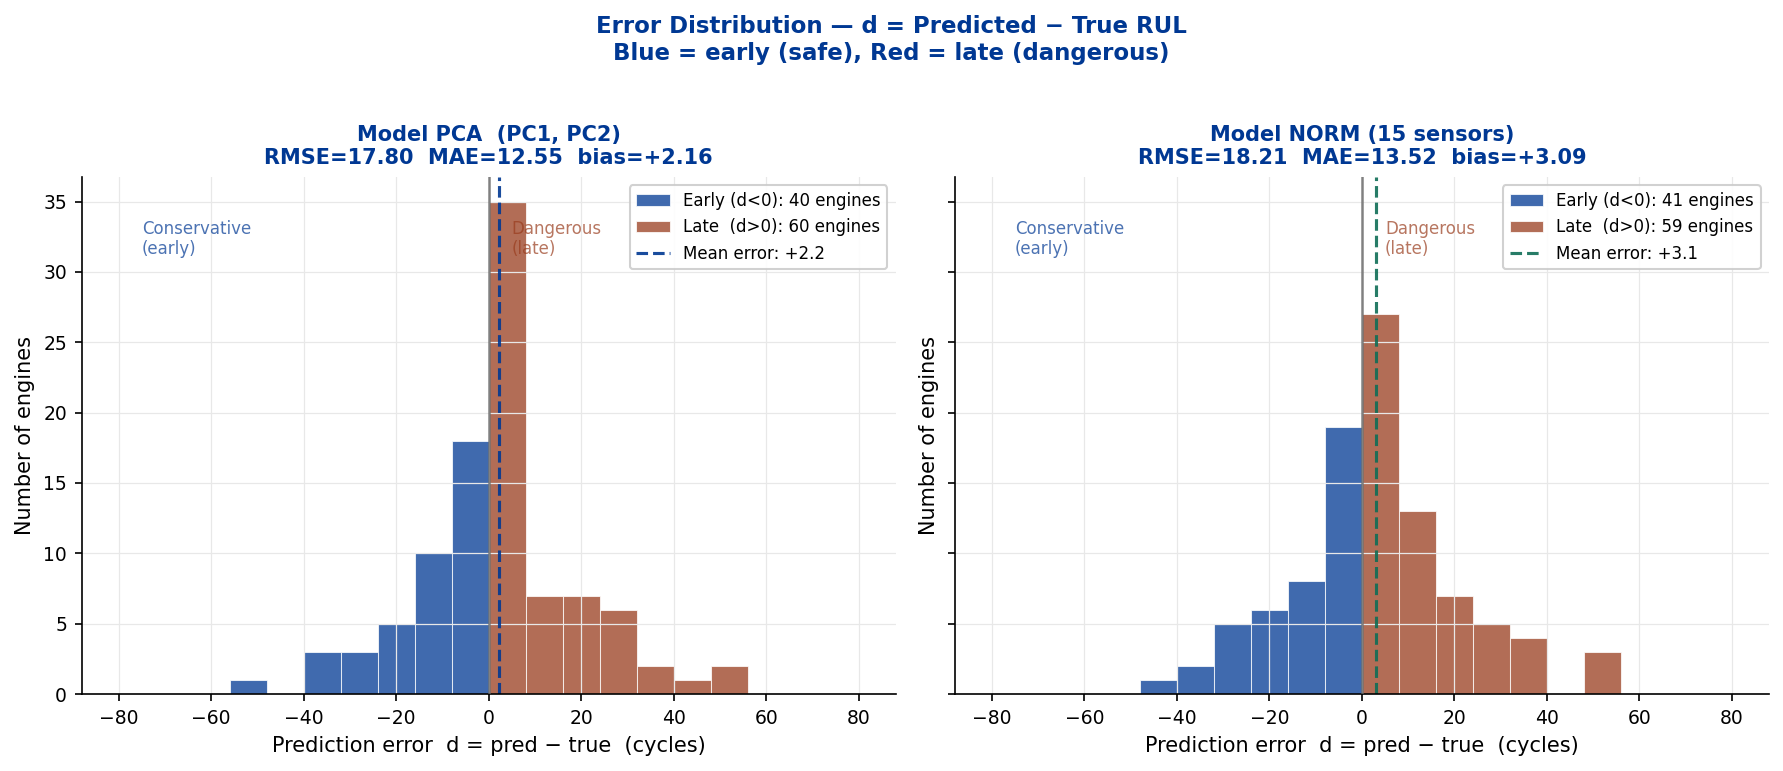
\includegraphics[width=\textwidth]{images/plot_B7_error_dist.png}

      \vspace{0.2cm}
      \begin{beamercolorbox}[sep=4pt]{block body}
\color{white}\small\centering
          \textbf{Best result: FD001\_PCA}\\
          RMSE = 17,80 cycles\\
          MAE = 12,55 cycles\\
          NASA Score = 815
\end{beamercolorbox}
    \end{column}
  \end{columns}
\end{frame}

% ── Slide 16: Terima Kasih ────────────────────────────────────────────────────
\begin{frame}[plain]
  \setbeamercolor{background canvas}{bg=uiblue}
  \centering
  \vspace{1.2cm}
  
\includegraphics[height=1.3cm]{images/logo_ui.png}

  \vspace{0.4cm}
  {\color{white}\LARGE\bfseries Terima Kasih\par}

  \vspace{0.3cm}
  {\color{uibluelight}\rule{0.5\textwidth}{0.4pt}\par}
  \vspace{0.3cm}

  {\color{white!80}\normalsize
    Luqman Alifio Arhab\\
    Azfa Rhazasta Abiandra\\
    Adamsyah Haryo Saksono\\
    Epsiarto Rizqi Nurwijayadi\par}

  \vspace{0.2cm}
  {\color{white!60}\small
    Departemen Teknik Mesin FTUI --- Data Analitik 2026\par}
\end{frame}

\end{document}
